From the criminal case data, we were able to build the network of \textit{Belonging Groups}. In this network, the nodes of those people whose roles are not referred to criminal actors are eliminated, such as: whistleblowers, victims, victims, etc. Figure \ref{fig:grafocompleto} shows a visualization of the network. In it, a graph made up of more than 30000 people with more Criminal Cases registered in the Coirón Management System can be observed (with the following criteria: involved in more than one case with the role of accused, suspected or denounced; deceased persons are included , minors and legal persons). In addition, all the relationships that exist between these people and their groups of belonging are displayed in the figure.

%A partir de los datos de los casos penales, pudimos construir la red de \textit{Grupos de Pertenencia}. En esta red, se eliminan los nodos de aquellas personas cuyos roles no sean referidos a actores delictivos, como ser: denunciantes, víctimas, damnificados, etc. En la Figura \ref{fig:grafocompleto} se muestra una visualización de la red. 
%En la misma se puede observar un grafo compuesto de más de 30000 personas con más Casos Penales registrados en el Sistema de Gestión Coirón (con los siguientes criterios: involucradas en más de un caso con rol de imputado, sospechoso o denunciado; se incluyen personas fallecidas, menores y personas jurídicas). Se visualizan además en la figura todas las relaciones que existen entre esas personas y sus grupos de pertenencia.
\vspace{-10pt}
\begin{figure}
	\centering
	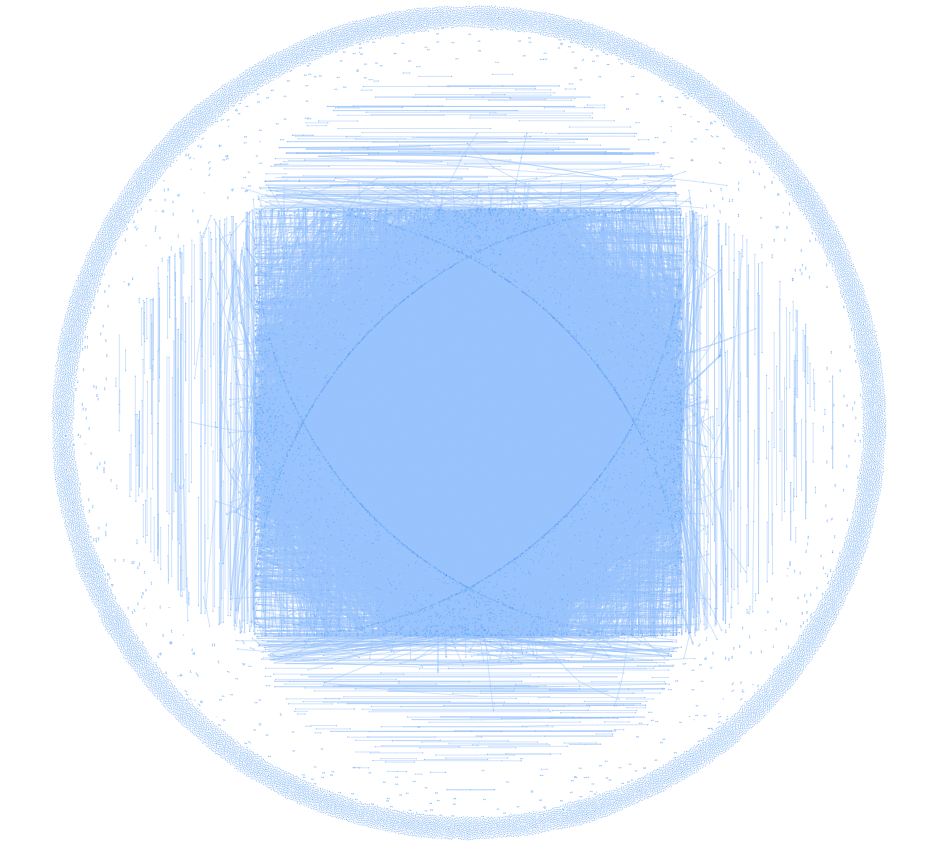
\includegraphics[width=0.4\linewidth]{grafo-30000-completo.png}
	\caption{More than 30000 people with more cases and their relationships.} 
	\label{fig:grafocompleto}
\end{figure}
\vspace{-10pt}
For the practical purposes of criminal investigation, a visualization with so many nodes and relationships is not representative or leads to any type of detection of criminal gangs, but it is a clear example of the universe of data that is available in the dataset used, as well as the power of the visualization tool. In Figure \ref{fig:grafosCompletos} you can see examples in which the membership groups of each node to be displayed have been taken into account, that is to say, the people with their particular membership groups are displayed (according to parameters of search selected). In image (a) 10000 people are shown, in (b) 1000 and in (c) 100 people with more cases and their related membership groups.
%A los sentidos prácticos de la investigación penal, una visualización con tantos nodos y relaciones no es representativa ni conduce a ningún tipo de detección de bandas delictivas, pero es un claro ejemplo del universo de datos que se disponen en el dataset utilizado, como así también la potencia de la herramienta de visualización. En la Figura \ref{fig:grafosCompletos} se pueden observar ejemplos en los que se han tomado en cuenta los grupos de pertenencia de cada nodo a mostrar, es decir que se visualizan las personas con sus grupos de pertenencias particulares (según parámetros de búsqueda seleccionados). En la imagen (a) se muestran 10000 personas, en (b) 1000 y en (c) 100 personas con más casos y sus grupos de pertenencia relacionados.
\vspace{-10pt}
\begin{figure}[htbp]
	\centering
	\subfigure[Top 10000.]{
		\begin{minipage}[t]{0.33\linewidth}
			\centering
			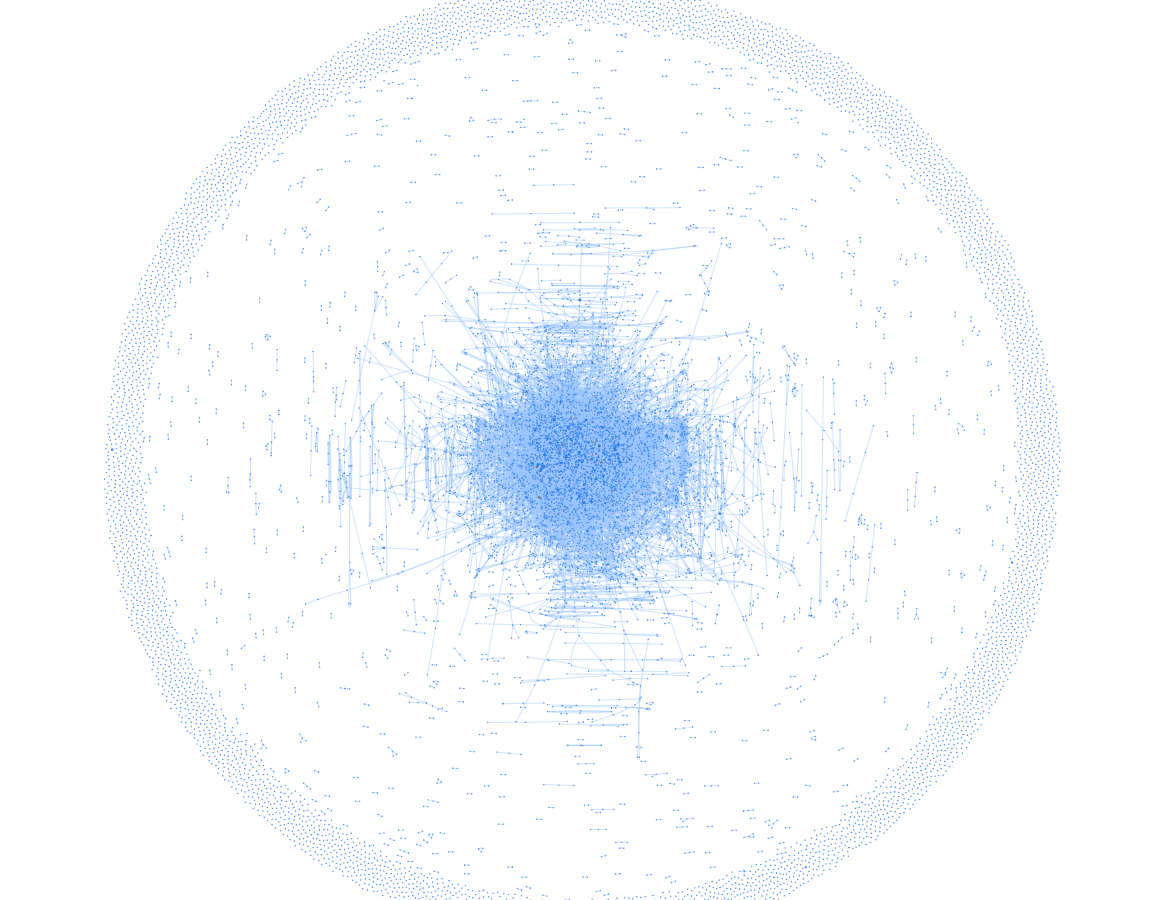
\includegraphics[width=1in]{grafo-10000-completo.png}
			%\caption{fig1}
		\end{minipage}%
	}%
	\subfigure[Top 1000.]{
		\begin{minipage}[t]{0.33\linewidth}
			\centering
			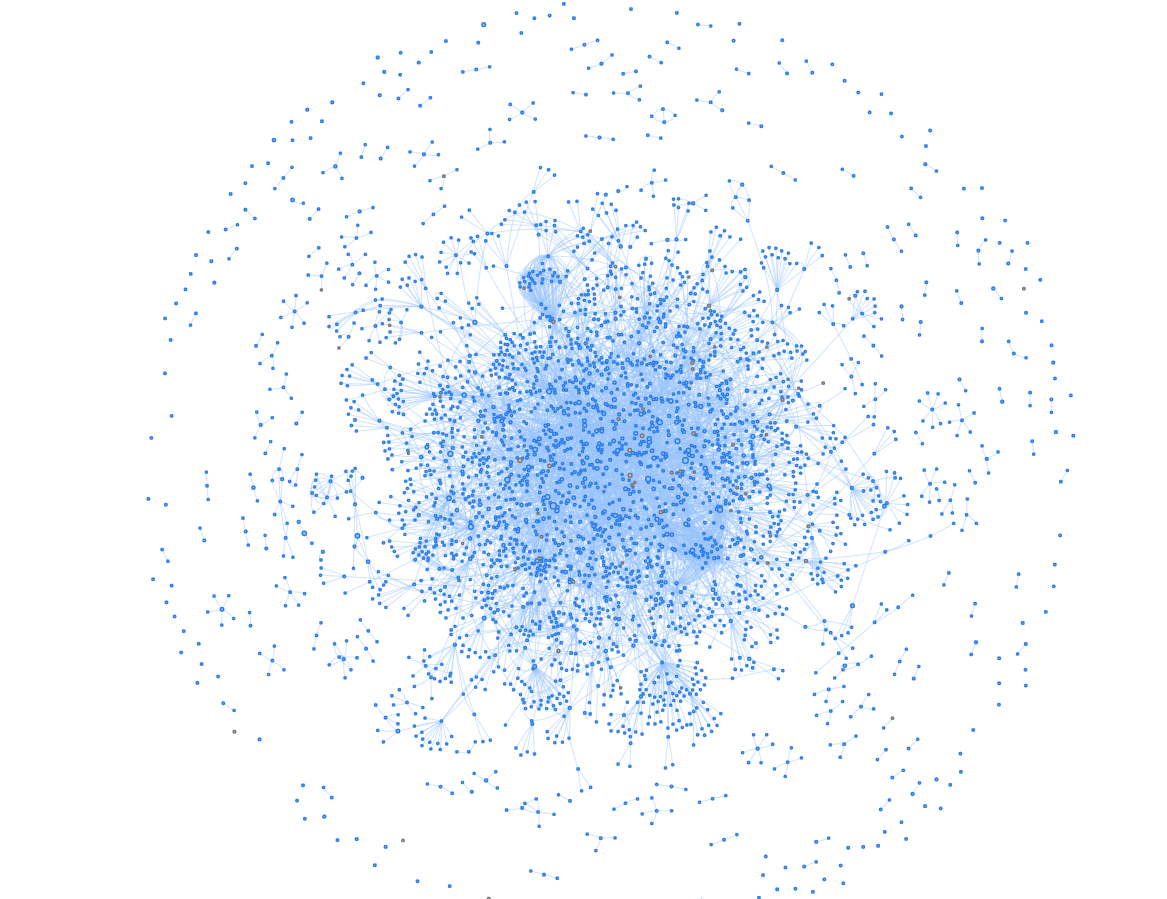
\includegraphics[width=1in]{grafo-1000-completo.png}
			%\caption{fig2}
		\end{minipage}%
	}%
	\subfigure[Top 100.]{
		\begin{minipage}[t]{0.33\linewidth}
			\centering
			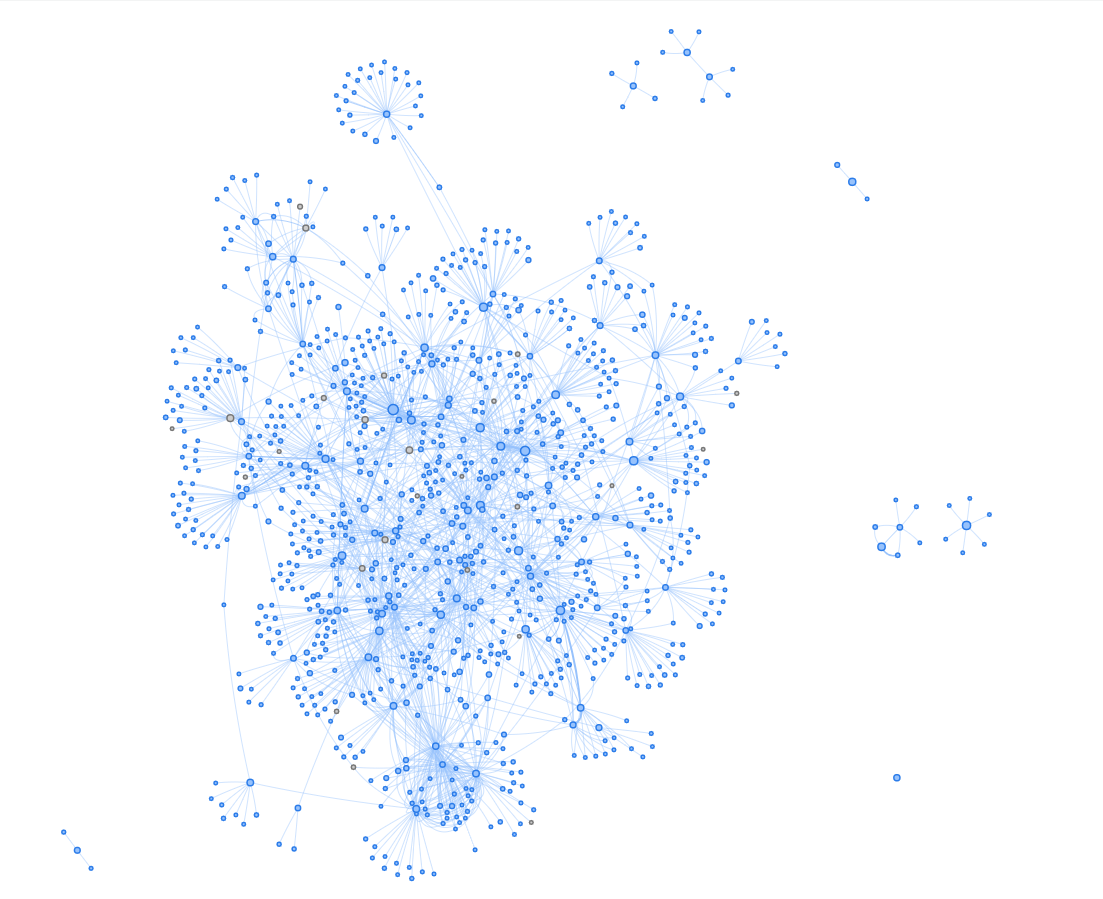
\includegraphics[width=1in]{grafo-100-completo.png}
			%\caption{fig3}
		\end{minipage}
	}%
	\centering
	\caption{ People in more cases, with the inclusion of their particular membership groups.}
	\label{fig:grafosCompletos}
\end{figure}
\vspace{-10pt}
By analyzing the composition of the network obtained, we can observe the relationships that exist between the nodes and how the graph is "balanced", making those nodes with few or no relationships remain on the periphery of the graph. In addition to this, the measure of centrality of those nodes that are surrounded by their related ones is also appreciable. A clearer approximation to denote the measure of centrality can be seen reflected in Figure \ref{fig:grafoTop10}, where only the 10 people with the most Cases and their belonging groups are displayed. Clearly, these 10 main nodes are surrounded by their membership groups and transitivities between them can be observed through nodes that are part of the membership group of more than one main node.
%Al analizar la composición de la red obtenida podemos observar las relaciones que existen entre los nodos y como se "equilibra" el grafo, haciendo que aquellos nodos con pocas o nulas relaciones queden en la periferia de la gráfica. Sumado a ello también es apreciable la medida de centralidad de aquellos nodos que son rodeados por sus relacionados. Una aproximación más clara para denotar la medida de centralidad puede verse reflejada en la Figura \ref{fig:grafoTop10}, en donde se visualiza sólo las 10 personas con más Casos y sus grupos de pertenencia. Claramente esos 10 nodos principales quedan rodeados de sus grupos de pertenencia y se pueden observar transitividades entre ellos a través de nodos que conforman parte del grupo de pertenencia de más de un nodo principal.
\vspace{-10pt}
\begin{figure}
	\centering
	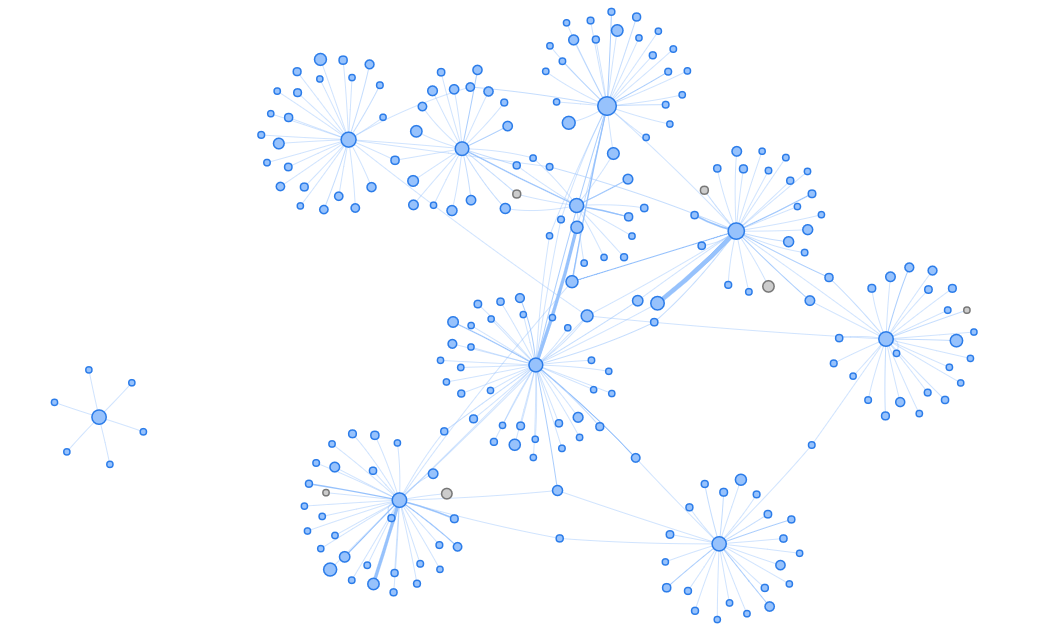
\includegraphics[width=0.5\linewidth]{grafo-10-completo.png}
	\caption{10 people with more cases in Coirón, with their relationships} 
	\label{fig:grafoTop10}
\end{figure}
\vspace{-20pt}
\subsubsection{Degree Centrality} 
%\subsubsection{Centralidad de Grado} 
Degree centrality is one of the simplest measures of centrality. In this, the number of links or connections that a node has with the other nodes belonging to a graph is measured. When an analysis of this type is applied, different measures can be determined. For example, in social networks we can measure the degree of entry of a node as the popularity or preference it has and the exit define it as an indicator of sociability. In our case study, members of criminal gangs dynamically modify their relationships with other members of the network, resulting in a change in their role and importance. A number of degree centrality measures can help identify these changes. These statistics can be used to filter the view of the network based on the value of a specific node and highlight its position within the network. The degree of centrality in our graph will then be defined as the number of direct links that an offender has. A node with a high degree can be seen as a "hub", an active and important node in the ~\cite{carley2006destabilization} network.
%La centralidad de grado es una de las medidas más simples de centralidad. En esta se mide el número de enlaces o conexiones que tiene un nodo con los demás nodos pertenecientes a un grafo. Cuando se aplica un análisis de este tipo pueden determinarse diferentes medidas. Por ejemplo, en redes sociales podemos medir el grado de entrada de un nodo como la popularidad o preferencia que posea y la salida definirla como un indicador de sociabilidad. En nuestro caso de estudio, los miembros de las bandas delictivas modifican dinámicamente sus relaciones con otros miembros de la red, lo que resulta en un cambio de su rol e importancia. Una serie de medidas de centralidad de grado pueden ayudar a identificar estos cambios. Estas estadísticas se pueden utilizar para filtrar la vista de la red en función del valor de un nodo específico y resaltar su posición dentro de la red. El grado de centralidad en nuestro grafo se definirá entonces como el número de enlaces directos que tiene un delincuente. Un nodo con un alto grado puede verse como un "centro", un nodo activo e importante en la red~\cite{carley2006destabilization}.
\vspace{-10pt}
\subsubsection{Transitivity} 
%\subsubsection{Transitividad} 
The clustering coefficient (transitivity) of a graph measures the degree of connection of a network. High clustering coefficients mean the presence of a high number of triangles in the network. It is well known in the literature ~\cite{wasserman1994social} that social networks show high clustering coefficient values when they reflect the underlying social structure of contacts between friends/acquaintances. 
Furthermore, high values of the local clustering coefficient are considered a reliable indicator of nodes whose neighbors are very well connected and between which a substantial amount of information can flow.
%El coeficiente de agrupamiento (transitividad) de un gráfico mide el grado de conexión de una red. Altos coeficientes de agrupamiento significan la presencia de un alto número de triángulos en la red. Es bien conocido en la bibliografía~\cite{wasserman1994social} que las redes sociales muestran valores altos del coeficiente de agrupamiento cuando reflejan la estructura social subyacente de los contactos entre amigos/conocidos. Además, los valores altos del coeficiente de agrupamiento local se consideran un indicador confiable de los nodos cuyos vecinos están muy bien conectados y entre los cuales puede fluir una cantidad sustancial de información.